\chapter{Bayesian survey and periodization of postembryonic CMZ activity}
\label{chap:CMZ}


\section{Postembryonic activity of the zebrafish CMZ}
It is useful to begin with a broad survey the population history of proliferative CMZ progenitors alongside a general measure of the increase in the volume of the cellular retina over time.  Fig. \ref{CMZoverall} presents estimates, calculated from sectional measurements as described in , of the overall population of the CMZ (Panel A), and the volume of the cellular retina (Panel B). Given the marginal posterior distributions of the mean population sizes, the probability of the mean population size at 60dpf being at least 3 times larger than the same parameter at 3 dpf is 

The overall picture is somewhat surprising; it seems that the CMZ undergoes a massive population buildup in the first month of life, a period of intense contribution to the neural retina in the second month of life, and a collapse in population during the third month, after which a modestly populated CMZ continues to make slow 

\begin{figure}[!h]
    \makebox[\textwidth][c]{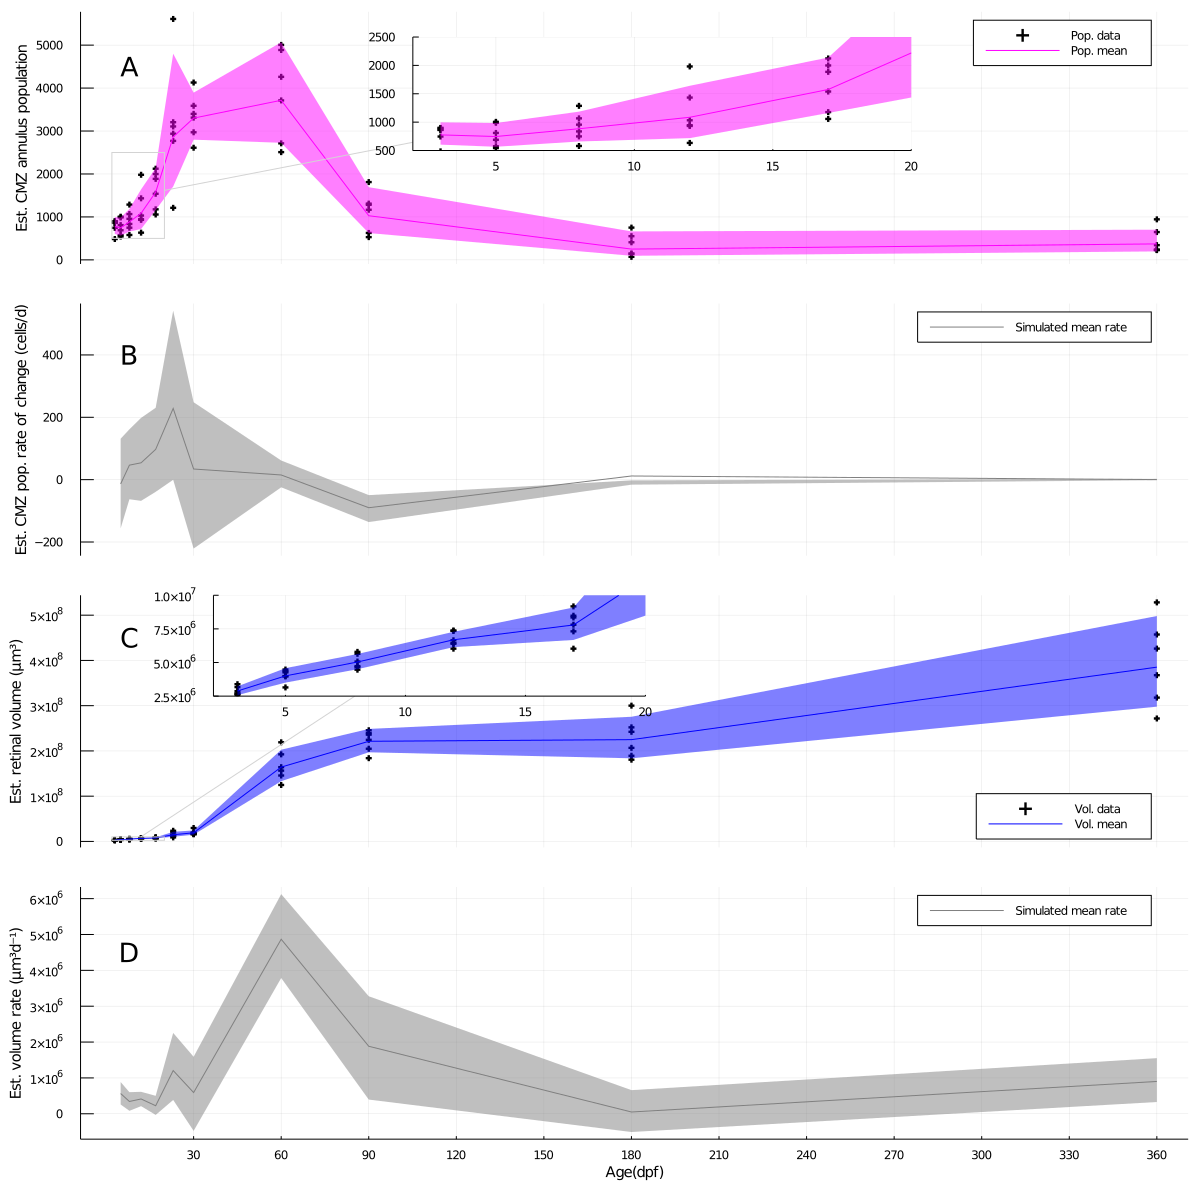
\includegraphics[width=1.2\textwidth]{cmz/CMZoverall.png}}    
    \caption{{\bf Population and activity of the CMZ over the first year of \textit{D.rerio} life}}
    Panel A: Marginal posterior mean CMZ annulus population. Panel B: Marginal posterior mean retinal volume estimate. Insets in Panels A \& B display data from 3-17 dpf. Panel C: Marginal posterior mean of the proliferative index of the CMZ annulus, assayed by specified retinal neurons with incorporated thymidine from an 8hr pulse at the indicated ages. Panel D: Mean daily rate of volumetric increase of the neural retina, calculated as the difference in volumes between two ages over the number of elapsed days. All means are displayed in a band representing the $\pm 95 \%$ credible interval for the marginal posterior distribution of the mean.
    \label{CMZoverall}
\end{figure}

\subsection{Population survey of the CMZ}

Before delving into the regional variation apparent in the population history of the CMZ's annulus, it will be useful to produce an overall estimate of the population of the CMZ annulus and an index of its overall proliferative activity. Because the analyses of population and activity data broken down by dorso-ventral and naso-temporal location refer to counts of cells in fixed-width sections, these figures do not account for the growing diameter of the CMZ. The individual population and activity datapoints presented in are derived from the lens diameter as detailed in \autoref{sec:lenspopest}. I calculated the marginal posterior distribution of the mean population size and activity index at each timepoint, assuming an uninformative normal-gamma prior distribution on the unknown mean and unknown variance of the normal gaussian models of these parameters. 



I first examined the mean size of dorsal and ventral populations of the CMZ, as ascertained by average counts of PCNA-positive cells at the retinal periphery in 14 $\mu$m central coronal sections of the eye. I calculated the marginal posterior distribution of the mean population size at the dorsal and ventral sides of for each timepoint, as described above. These data are presented in Fig. \ref{DVontology}.

\begin{figure}[!h]
    \makebox[\textwidth][c]{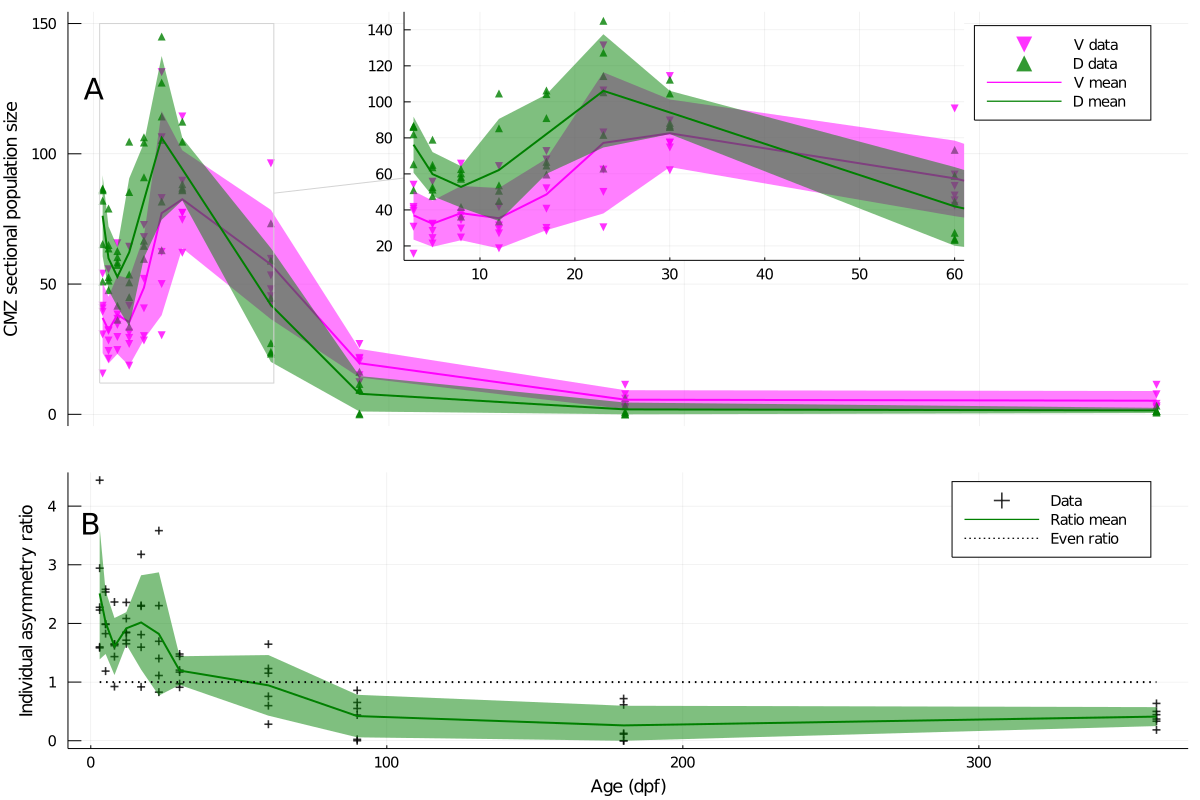
\includegraphics[width=1.2\textwidth]{cmz/DVontology.png}}    
    \caption{{\bf Developmental progression of dorso-ventral population asymmetry in the CMZ.}}
    Marginal posterior distribution of mean dorsal (D) and ventral (V) population size in 14$\mu$m coronal cryosections (panel A) or intra-individual D/V count asymmetry ratio (panel B), $\pm 95\%$ credible interval, n=5 animals per age. Data points represent mean counts from three central sections of an experimental animal's eye. 
    \label{DVontology}
\end{figure}

\begin{figure}[!h]
    \makebox[\textwidth][c]{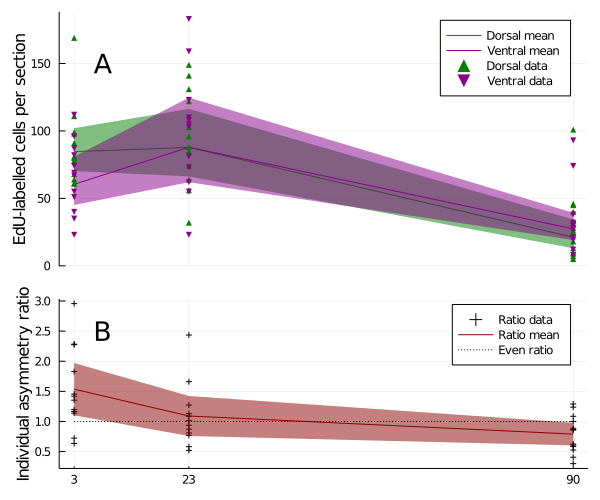
\includegraphics[width=1.2\textwidth]{cmz/DVcontribution.png}}    
    \caption{{\bf Developmental progression of dorso-ventral asymmetry in CMZ contributions to the neural retina.}}
    Marginal posterior distribution of mean dorsal (D) and ventral (V) population size in 14$\mu$m coronal cryosections (panel A) or intra-individual D/V count asymmetry ratio (panel B), $\pm 95\%$ credible interval, n=5 animals per age. Data points represent mean counts from three central sections of an experimental animal's eye. 
    \label{DVcontribution}
\end{figure}


\section{Toward computational models of the CMZ}